\section{Systems description} \label{sec:methods}

\textbf{giancarlo modifications: I've changed a little bit the structure to create a kind of flux over the contents. The main idea is to switch the mind set from METHOD $\rightarrow$ (CLASSIFICATION) SYSTEM, in this way we can report our work from a software engineer point of view, analysing each part/process as a module. It seams stupid, but in this way I have a name fro each step of the METHOD/SYSTEM and I suppose can help the readers to better understand what we have done.}


In this section we are going to describe the tweets classification systems built, from a module perspective we can describe our systems as composed of three main blocks: text pre-preprocessor (\cref{subsec:preprocessing}),  text representation (\cref{subsec:representation}) and classification model (\cref{subsec:classificationModel}). 


\subsection{Initial investigation} \label{subsec:boh}
To address the tweets classification problem we began our investigation analysing some of the most widely used text representations and classifiers.
We began analysing possible text representations focusing our attention on lexical features based: \emph{Bag Of Words} \cite{harris1954distributional},\emph{Bag Of N-Grams} (bigrams and trigrams), both with and without \emph{term frequency-inverse document frequency} normalization (i.e. TF-IDF norm).
Regarding possible classifiers exploiting above representations,  we analysed \emph{Random Forest, Decision Trees, Support Vector Machines} and \emph{Multi Layer Perceptron}, but since the results obtained with the combination of those \emph{model + representation} were outperformed by neural network based models, we decided not to report their analysis in this paper, but rather focus the modules description in relation to neural models.


\subsection{Text Preprocessor} \label{subsec:preprocessing}


We explored different combinations of twitter pre-processing, as converting some elements such mentions, emoji, smiley, hashtags into constant string (i.e. Tokenize @Ambros and \#atoppe :) $\rightarrow $ Tokenize \$MENTION and \$HASHTAG \$SMILEY ); removeing elements as URLs, reserved words and numbers.
We also measured the contribution of stemming, stopwords and punctuation removal.
To address those pre-processing we used the following \cite{nltk} \cite{tweets-preprocessor}.

\subsection{Text representation} \label{subsec:representation}
As a tweet representation used as first layer

To represent to tweet fed into the classifier we decided to used word embeddings,which is a tecnique where elements (in our case words and n-grams) are mapped into a vector of real numbers.
The whole sentence is mapped into a matrix with dimension \emph{sentence lenght} $\times$ \emph{embedding dimension}.
We left the sentence length as a parameter and the best results were obtained with length=30, that's reasonable since the average tweet length in words in 24.
If the sentence dimension is bigger than the selected window we used the first length words, if the sentence is smaller than the windwos we used 0-right padding.

\subsubsection{Words vectors}
Since the number of tweets is considered small to learn vector representation of words, we tried to initialize the embedding matrix with pretrained word vectors.
In particular we used vectors trained on wikipedia using fastText \cite{bojanowski2016enriching}.
We tried static pretrained vectors, learning them during training starting from a random matrix or from the pretrained embeddings.

\subsubsection{N-gram embedding}
We also tried to learn an embedding for n-grams (bigrams and trigrams), but, since the corpus is small, n-grams frequencies are very low and the algorithm is not able to learn a valid embedding.
Also there are no pre-trained n-grams embeddings available.
Bigrams brought a small improvement, bigger n-grams result in performance decrease.



\subsection{Classification models} \label{subsec:classificationModel}
In the following section we present different neural network models, each model has as first layer an embedding layer that maps words to the corresponding word vectors, as described in the previous section.


\subsubsection{Convolutional Neural Network}
Convolutional Neural Networks are considered state of the art in many text classification problem. (GIANCARLO, citazioni?)
This model is composed by a convolutional layer, followed by a global max pooling layer and two fully conncted layers.

\subsubsection{Long short-term memory}
LSTM is a type of Recurrent Neural Network that is relatively insensitive to gap length, compared to others RNN, they are considered state of the art in many NLP topics, like machine translation.
In this model the classical embedding layer is followed by an LSTM layer with 128 units, terminated by a fully connected layer.
We also tried Bidirectional LSTM, since they are bringing an improvement in different tasks, but they are performing worst on our use case.

\subsubsection{Fast text}
This model is based on this paper \cite{joulin2016bag}.
Differently to the other models where just words are used, here Bag of n-grams are added to the imput as  additional features to capture some partial information about the local word order.
It this model the embedding output is directly fed into a GlobalAveragePooling layer, that transofrms the whole sentece in a single vector computed as the average of the word vectors.
This vector is then projected into 2 fully connceted layers. In the paper the number of hidden layers is fixed to 10, but we measured better performance using just 2 layers.
\begin{figure}[h]
\centering
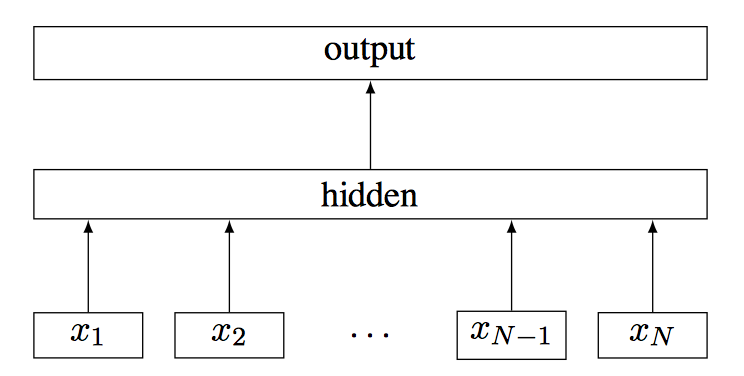
\includegraphics[width=.75\columnwidth]{fast_text}
\caption{Model architecture of fastText for a sentence with N ngram features x1 , . . . , xN . The features are embedded and averaged to form the hidden variable.}
\label{fig:ants_example}
\end{figure}
\textbf{@ Luca: Source: \cite{joulin2016bag }


\subsubsection{KIM.}

\textbf{@ Luca: Source: Zhang, Y., & Wallace, B. (2015). A Sensitivity Analysis of (and Practitioners’ Guide to) Convolutional Neural Networks for Sentence Classification.}
\textbf{http://www.wildml.com/2015/11/understanding-convolutional-neural-networks-for-nlp/}

\begin{figure}[h]
\centering
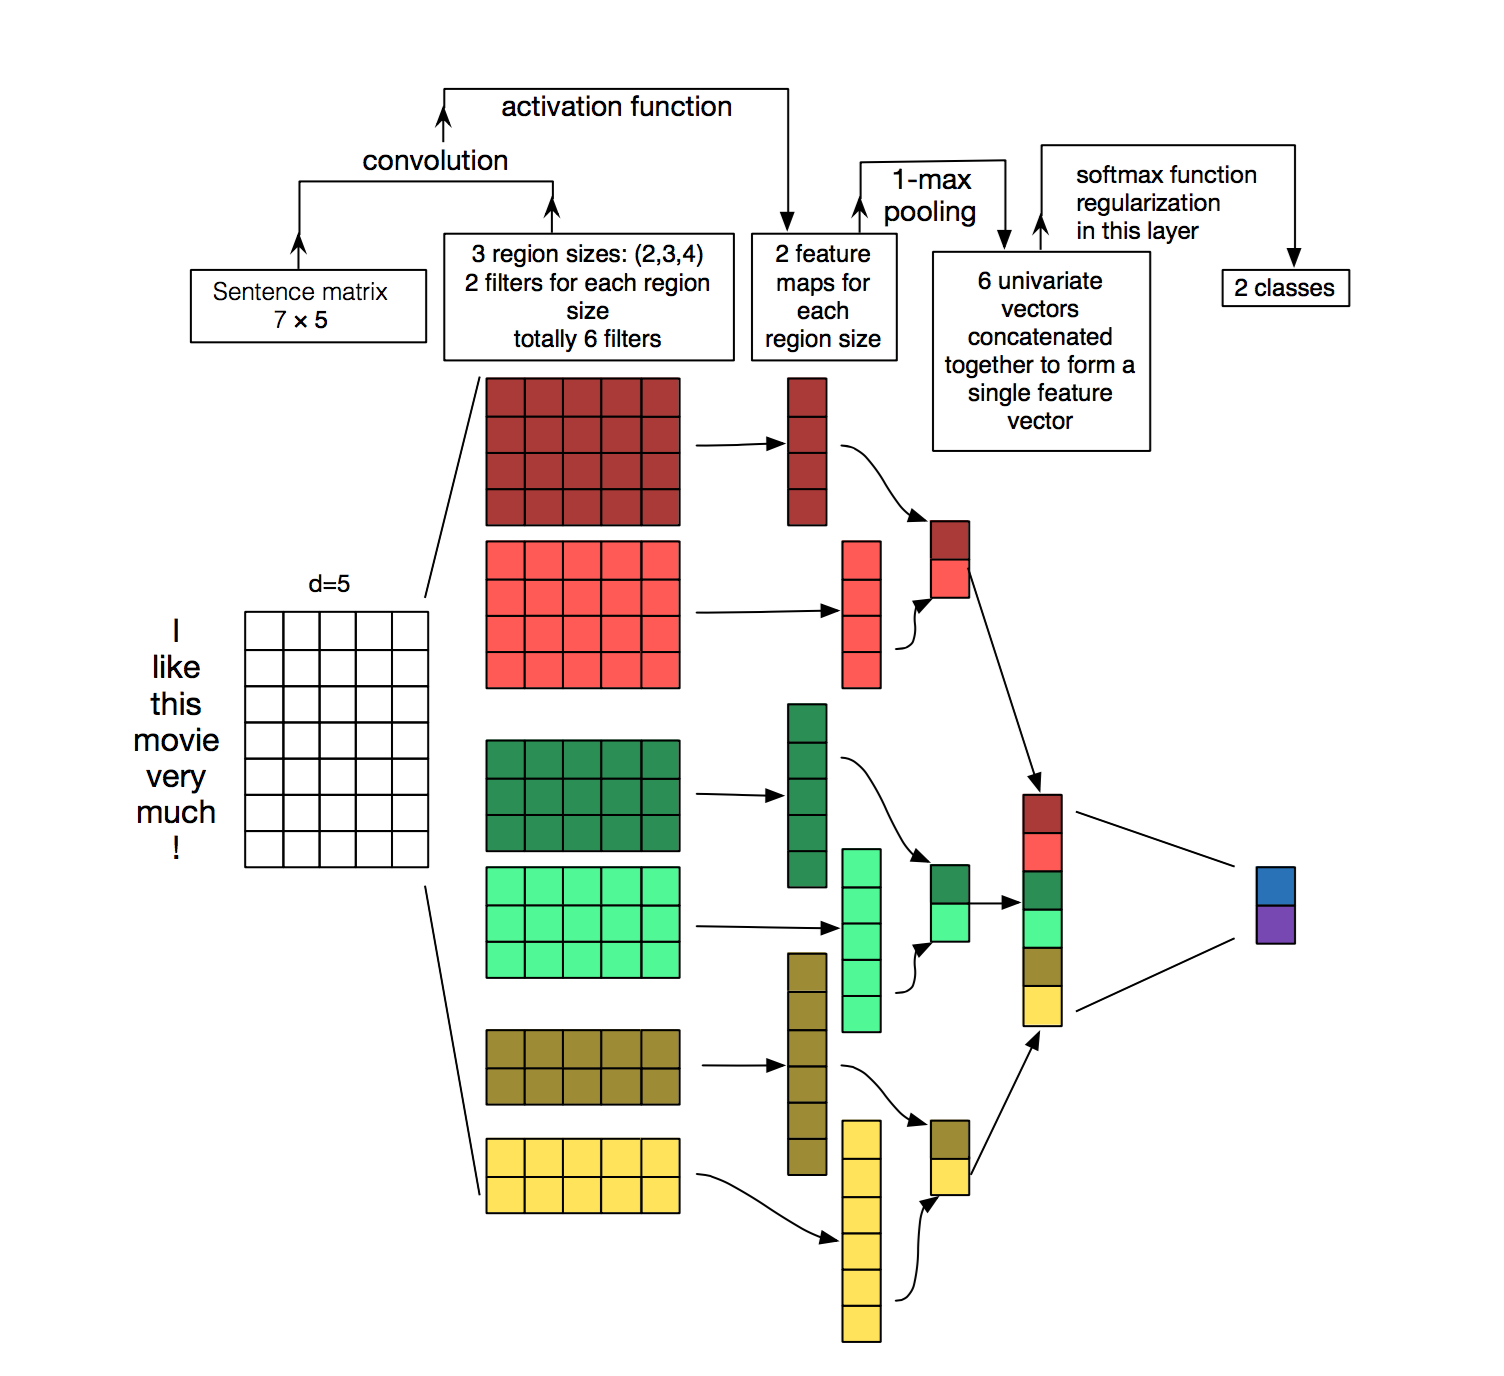
\includegraphics[width=.75\columnwidth]{kim_cnn}
\caption{Illustration of a Convolutional Neural Network (CNN) architecture for sentence classification}
\label{fig:ants_example}
\end{figure}
\textbf{@giancarlo: Non penso che ants_example vada esattamente qui :D}


This model is based on this paper \cite{kim2014convolutional}. It is based on different filter region size convolutions, followed by maxpooling layers.
All those outputs are concatenated to build sentence representation that is finally projected into a dense layer for the classification.
The intuition behind this model is that smaller filter region size should be able to capture short sentence patterns (similar to ngrams), while bigger sizes should capture sentence level features. We reached the best performance using [2, 3, 5, 7] as filter sizes.
